\section{Motivation}

In order to ensure the ground-handling employees work at their optimal performance, their individual motivation must be accounted for. Studies on this subject argues that; \"intrinsic motivation (based in interest) and autonomous extrinsic motivation (based in importance) are both related to performance, satisfaction, trust, and well-being in the workplace\" (Self-determination theory and work motivation, MARYLE'NE GAGNE AND EDWARD L. DECI).

\begin{figure}
\centering
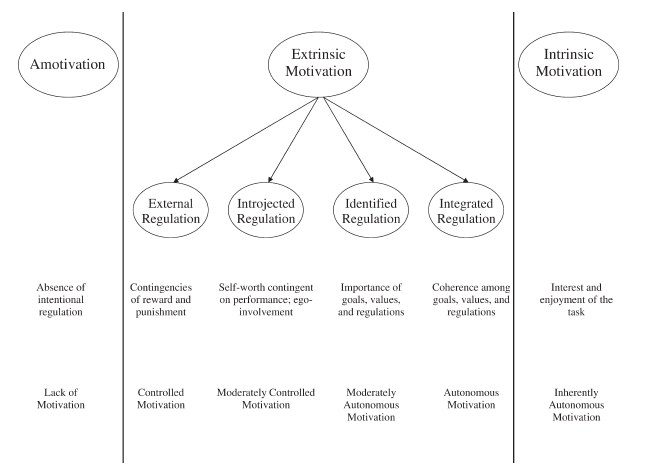
\includegraphics[width=\pagewidth]{Grafik/Motivation}
\caption{text}
\label{Hackman}
\end{figure}

It is important to maintain autonomous intrinsic motivation that an employee level of specific competence matches the requirements for that specific task, the task must not be too difficult or too simple. Failing to meet this will result in amotivation toward certain task because not really what one is doing or feeling too competent. Although tasks will incur in a groundhandling environment, an extrinsic motivation can promote autonomous behavior to get a raise or so the boss wont become upset.

\begin{figure}
\centering
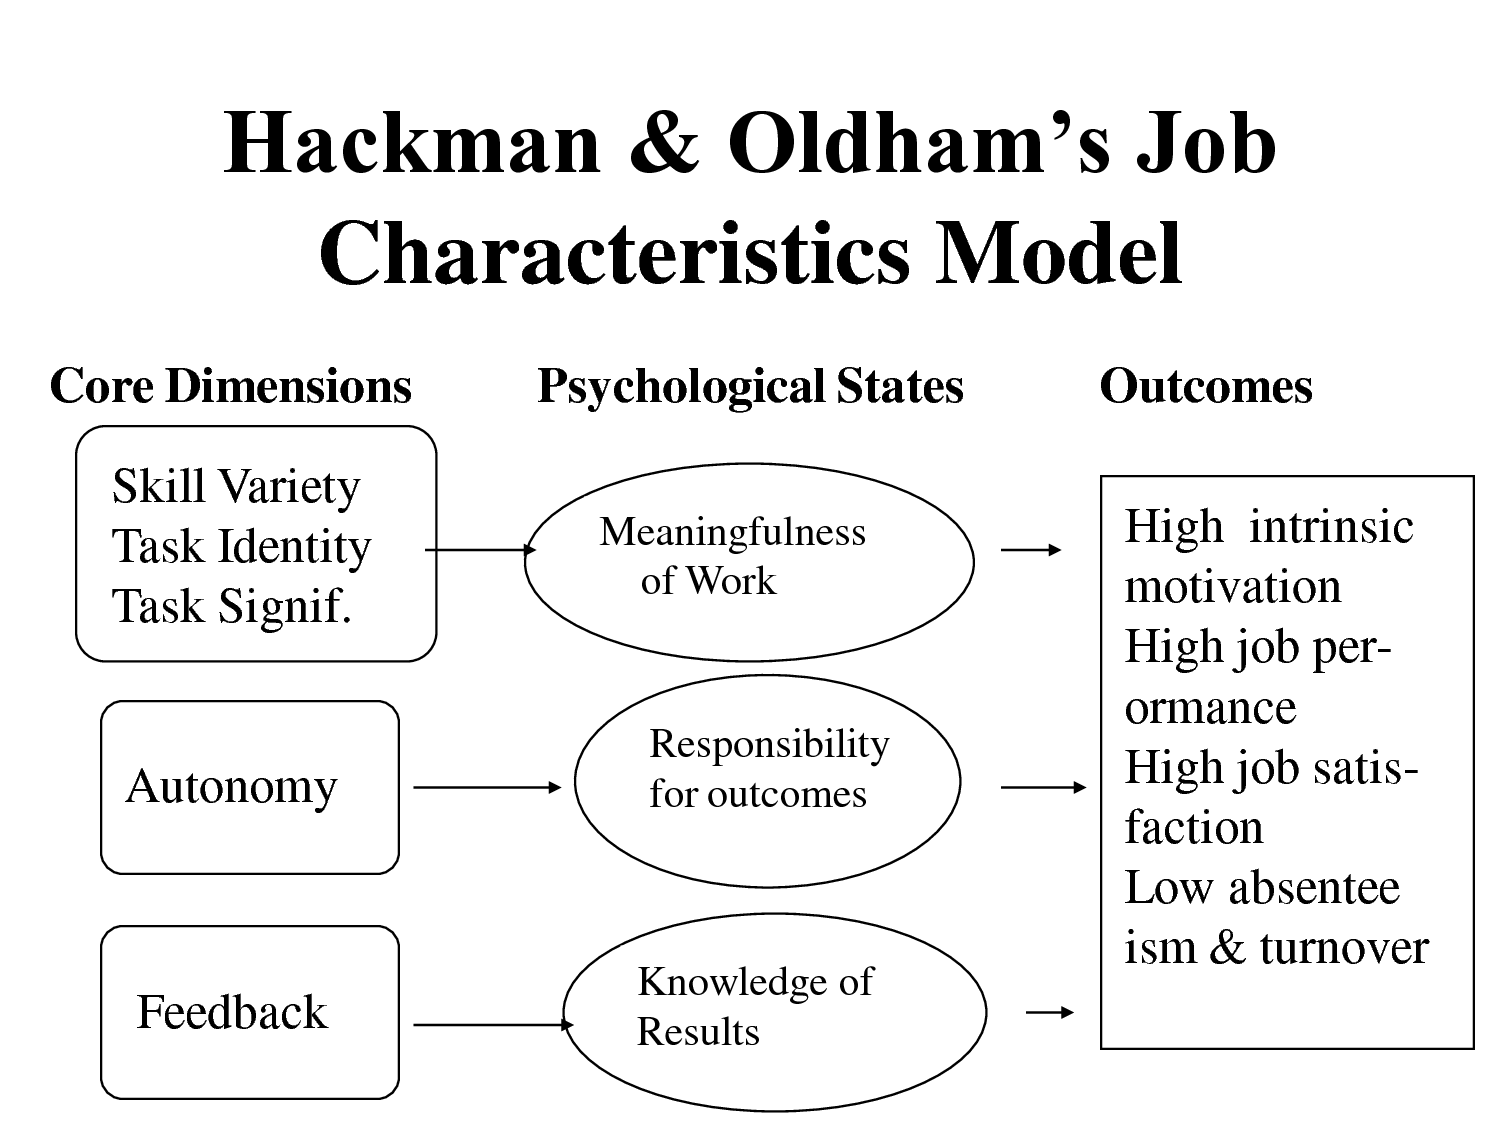
\includegraphics[width=\pagewidth]{Grafik/Hackman}
\caption{text}
\label{Hackman}
\end{figure}


A model of job characteristic introduced by Hackman and Oldman, which suggested the most effective factors of building motivation is through optimal job design. (Hackman and Oldman)

\begin{itemize}
\item provide variety, involve completion of a whole, and have a positive impact on the lives of others;
\item afford considerable freedom and discretion to the employee (what action theorists refer to as decision latitude); 
\item provide meaningful performance feedback.
\end{itemize}

Constructive feedback can influence autonomous motivation, but it also suggests that the supervisors and managers are important in creating a work environment, consisting of a mix of intrinsic motivation and extrinsic motivation, which is superior in situations that include both complex tasks that are interesting and less complex tasks that require discipline. 
